\chapter{Interpreting a Linear Regression Model \label{chapter:linreg}}

This chapter is devoted to understanding the structure of linear regression models. We first encountered them in Chapter~\ref{chapter:regression} as ``just one example'' of a regression model. However, linear regression's overwhelming popularity in the clinical domain means that one cannot do clinical data science without fully understanding these models' structure and how to interpret the output produced by model fitting software. 

%%%%%%%%%%%%%%%%%%%%%%%%%%%%%%%%%%%%%%%%%%%%%%%%%%%%%%%%%%%%%%%%%%%%%%%%%%%%%%%%

\section{Biomarker Example from Chapter~\ref{chapter:regression}}

In Chapter~\ref{chapter:regression}, we saw an example where information about two predictors -- a disease severity score ($x_1$) and a social determinants score ($x_2$) -- was used to predict the level of a disease recurrence biomarker. One of the three supervised learning algorithms we tried was a \textbf{linear regression} model (Section~\ref{ssect:linreg}). The output from that model is repeated below.
\begin{center}
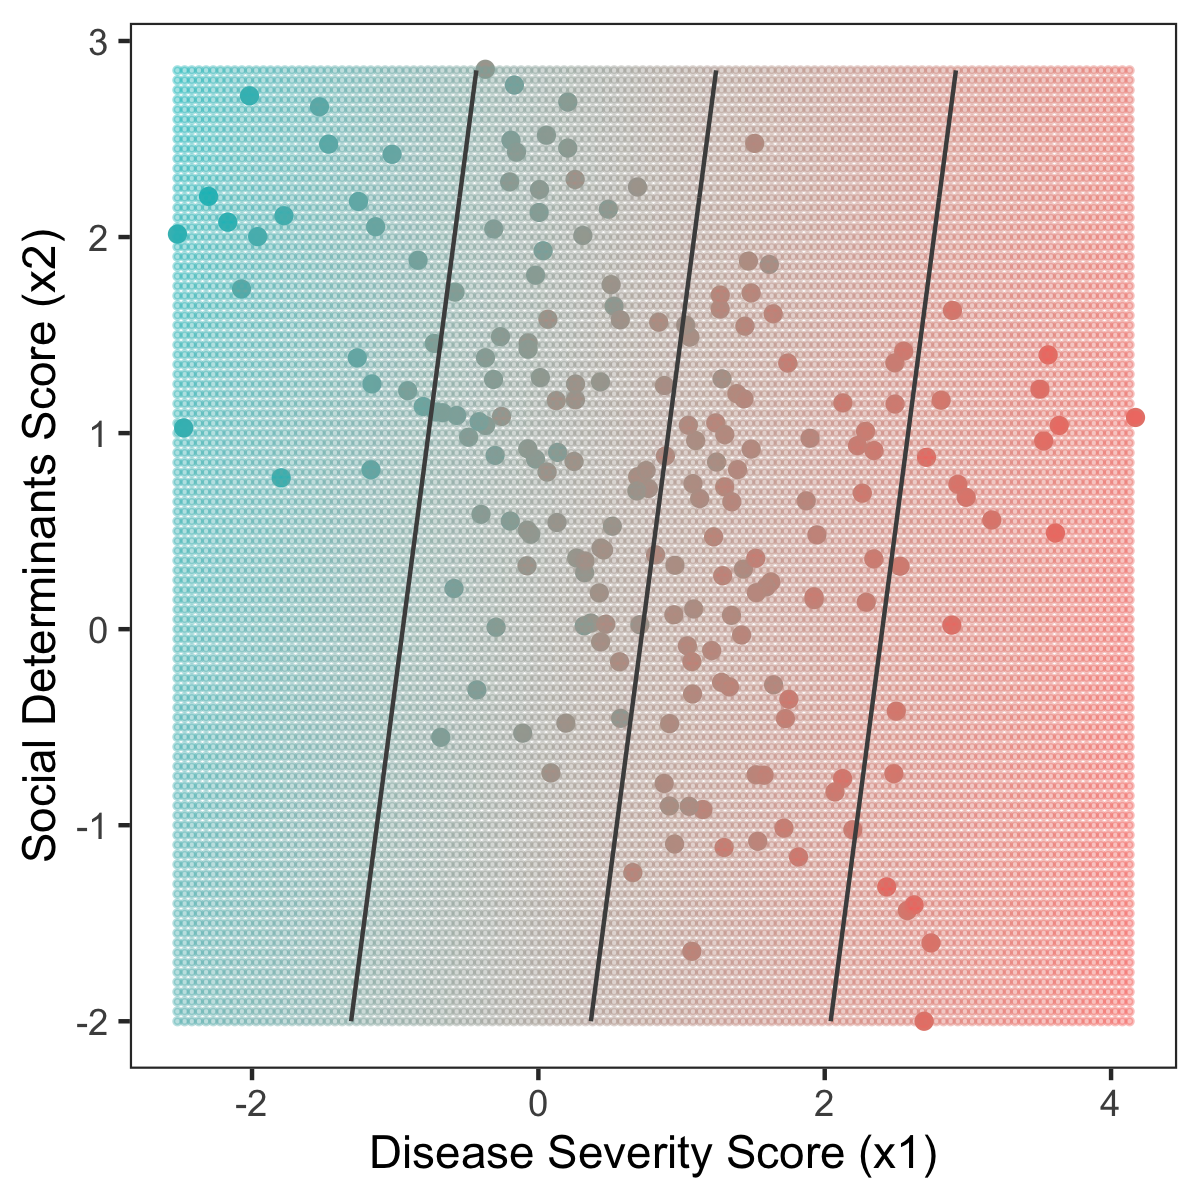
\includegraphics[width=0.35\textwidth]{img/esl-reg-linear.png}
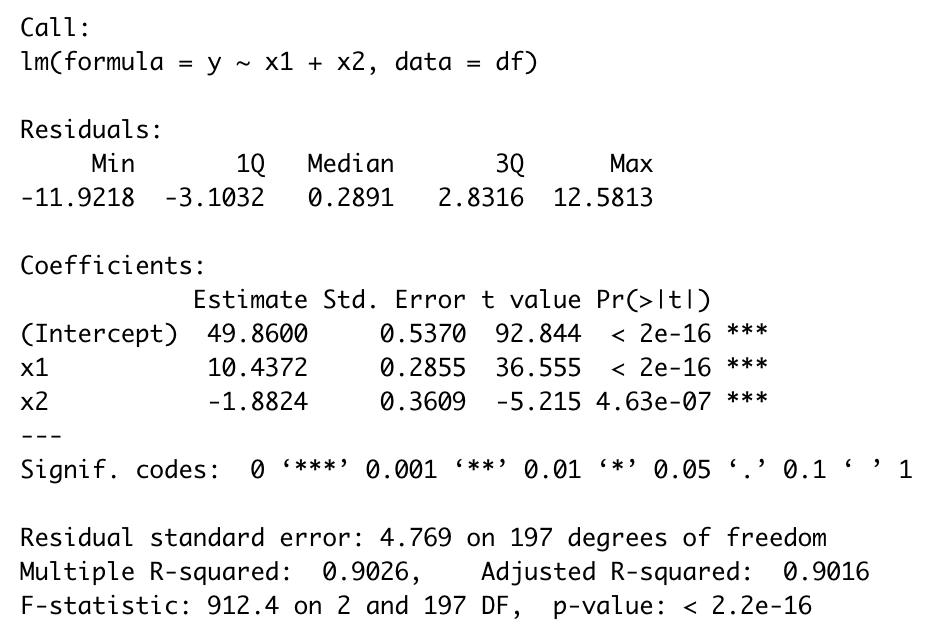
\includegraphics[width=0.64\textwidth]{img/linear-regression-model-output.png}
\end{center}

\begin{question}{}
What are the number of samples, $n$, and the number of predictors, $p$, for this dataset?
\end{question}

\noindent But what do all these numbers \emph{mean}?

%%%%%%%%%%%%%%%%%%%%%%%%%%%%%%%%%%%%%%%%%%%%%%%%%%%%%%%%%%%%%%%%%%%%%%%%%%%%%%%%

\section{Understanding the Model Summary}

A linear regression model looks like this (see also Chapter~\ref{chapter:regression}, Section~\ref{ssect:linreg}):
$$ y = \beta_0 + \beta_1 x_1 + \dots + \beta_p x_p + \varepsilon $$
where we assume that the error, $\varepsilon$, is normally distributed, $\mathcal{N}(0, \sigma)$. Another way of saying this is that we are assuming the outcome, $y$, is normally distributed with mean $\beta_0 + \beta_1 x_1 + \dots + \beta_p x_p$ and standard deviation $\sigma$. 

\subsection{The Call}

The first line of the output is just repeating the call you made to the \verb|lm| function in R to fit the model. The \texttt{lm} package fits linear regression models using ordinary least squares. However, linear regression models are also a type of generalized linear model (see Chapter~\ref{chapter:glms}) and can be fit using maximum likelihood. In R, if you use the \texttt{glm} package with \texttt{family = "gaussian"} you should get identical coefficients and error estimates to what you get using the \texttt{lm} package.

\subsection{The Residuals}

A \textbf{residual} is a measure of how much the true outcome value ($y$) of one datapoint differs from the model's prediction. For a linear regression model, the residual of training point $i$ is:
$$ \text{residual}^{(i)} = y^{(i)} - \hat{y}^{(i)} $$
where $\hat{y}^{(i)}$ is the model's prediction:
$$ \hat{y}^{(i)} = \beta_0 + \beta_1 x_1^{(i)} + \dots + \beta_p x_p^{(i)}. $$
Here is a histogram of the residuals for this model:
\begin{center}
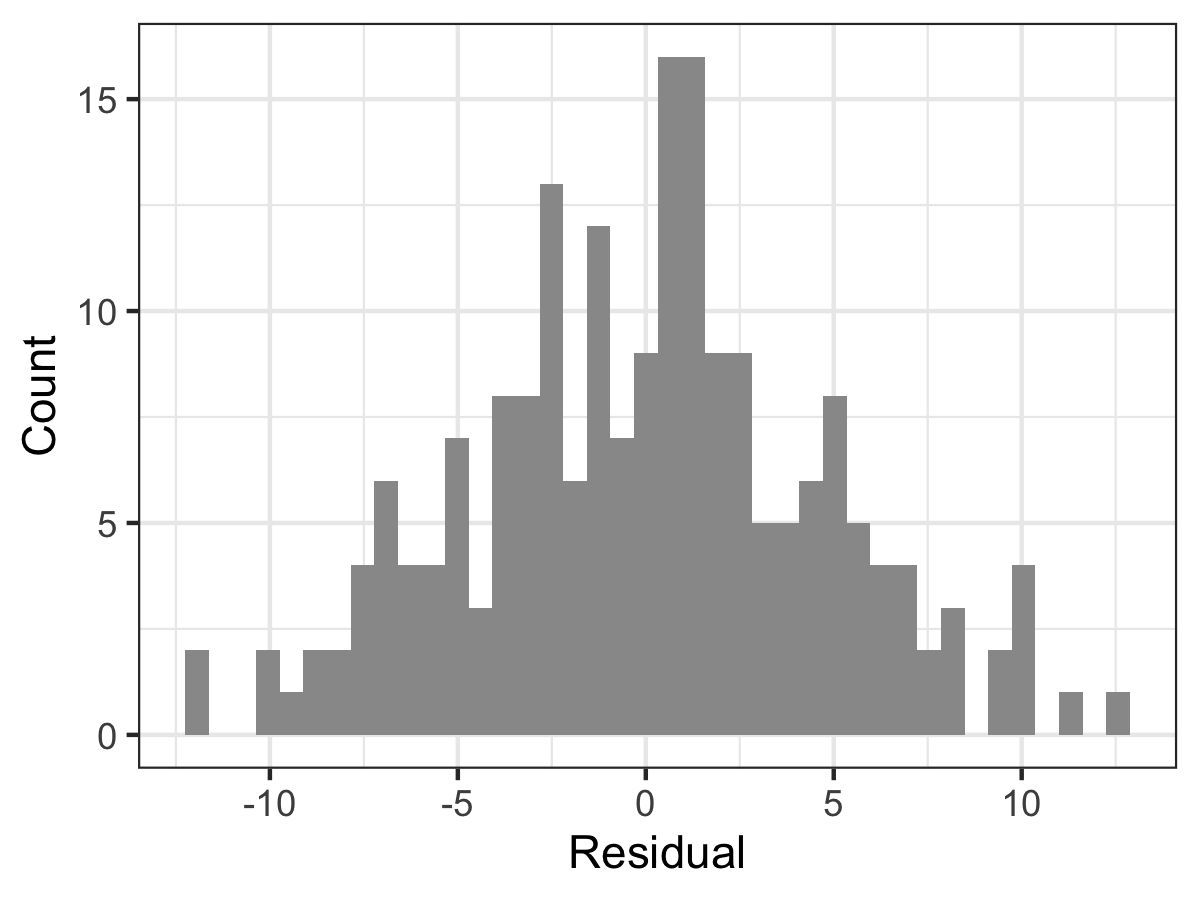
\includegraphics[width=0.7\textwidth]{img/linreg-example-residuals.png}
\end{center}

\begin{question}{}
Estimate the maximum, minimum, and mean residuals from this graph. Do they match what is in the model output?
\end{question}

The residuals play an important role in linear regression models because they are what allow us to estimate $\sigma$. They also play an important role in model diagnostics because they enable us to check one of the core model assumptions: the assumption that $\sigma$ is constant. We can check this assumption by making a plot of the residuals vs. $\hat{y}$:
\begin{center}
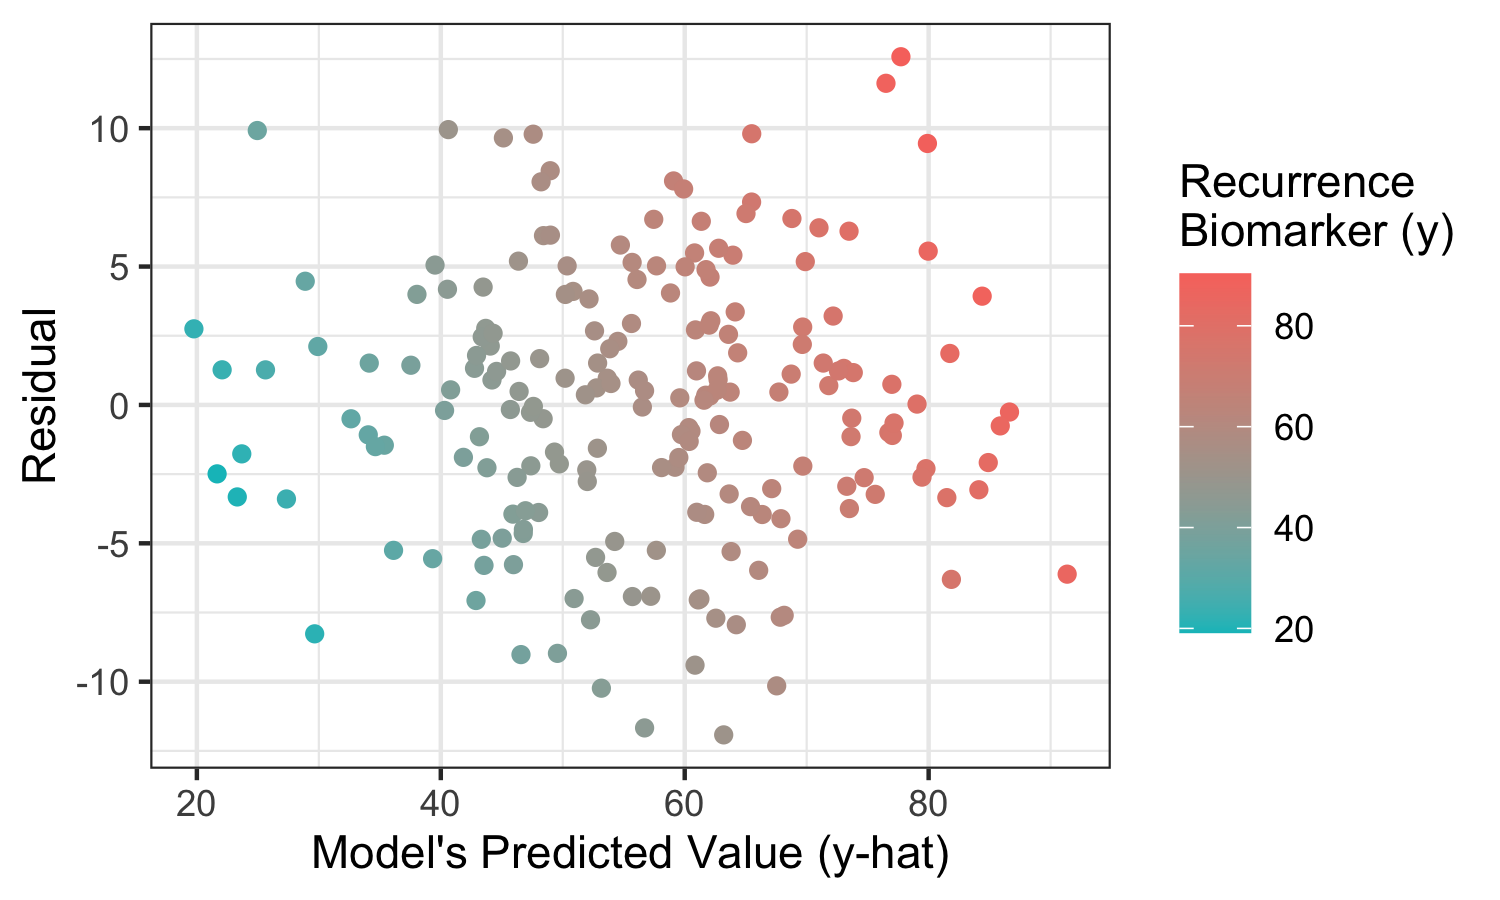
\includegraphics[width=0.7\textwidth]{img/linreg-example-residual-vs-fitted.png}
\end{center}
We can also check the normality of the residuals by making a plot of their values vs. what we would expect if the residuals were perfectly normally distributed with the same mean and standard deviation:
\begin{center}
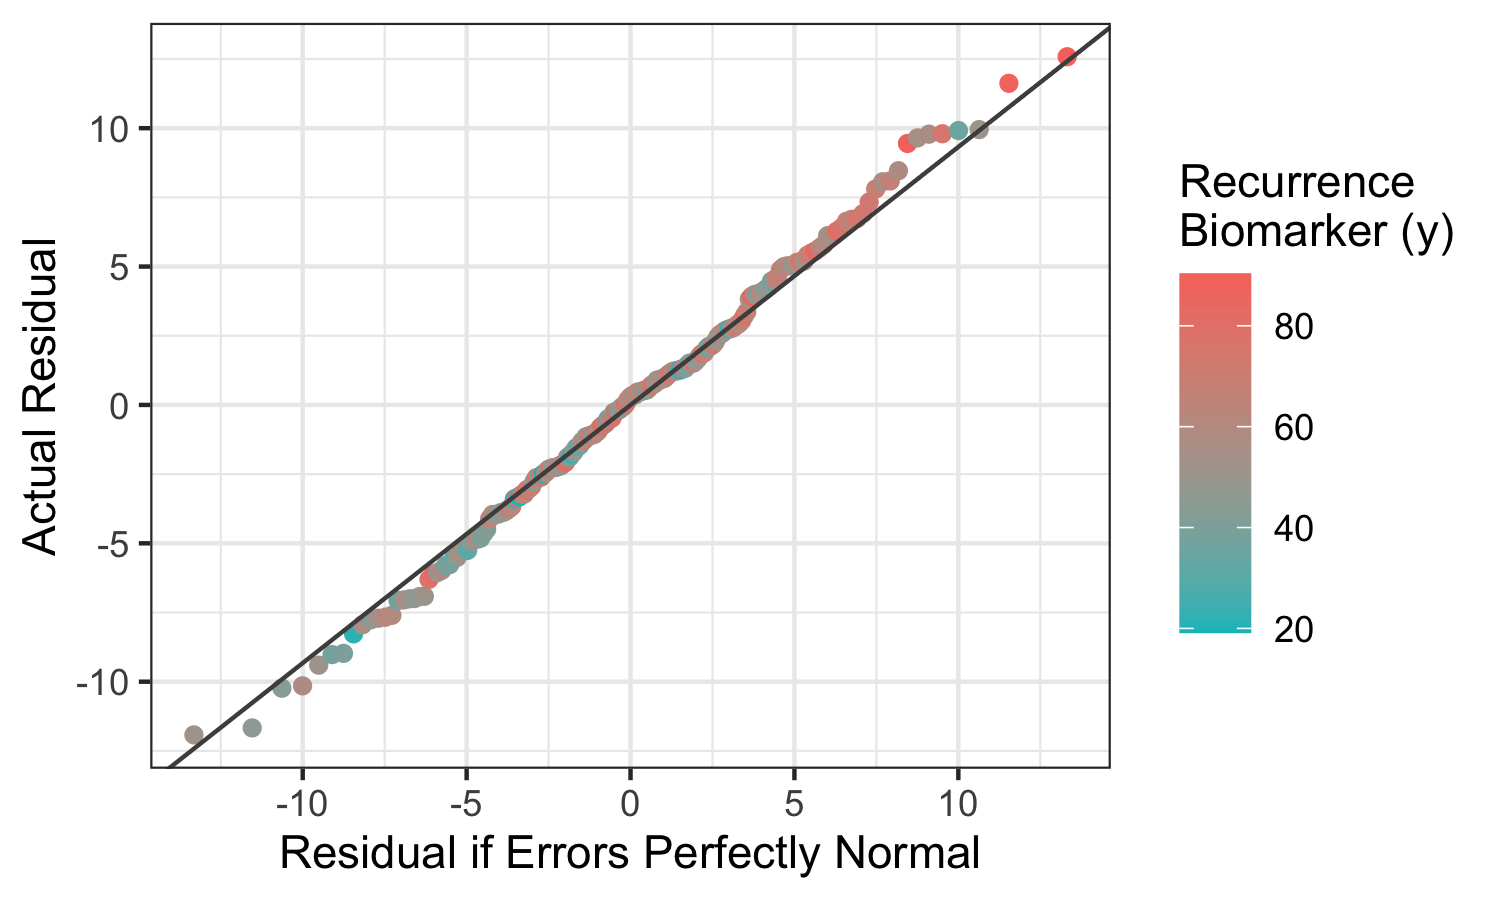
\includegraphics[width=0.7\textwidth]{img/linreg-example-almost-qq-plot.png}
\end{center}
This is not quite a \textbf{QQ-plot}, one of the standard diagnostic plots of linear regression, because it's plotting the actual values of the residuals instead of their quantiles. But aside from the axis scales, it's exactly the same. We'll see formal QQ-plots later. 

The fact that the points in the second plot lie close to a line is a good indication that the residuals are normally distributed. Another thing to notice from this plot is that the colors of the points (their $y$ values) are unrelated to their residuals. 
\vspace{5mm}

\begin{question}{}
The four plots below show a famous dataset called \textbf{Anscombe's quartet}. The regression lines produced by fitting a linear regression model to each dataset are identical, but only one dataset actually fulfills the assumptions of a linear regression model. 
\begin{center}
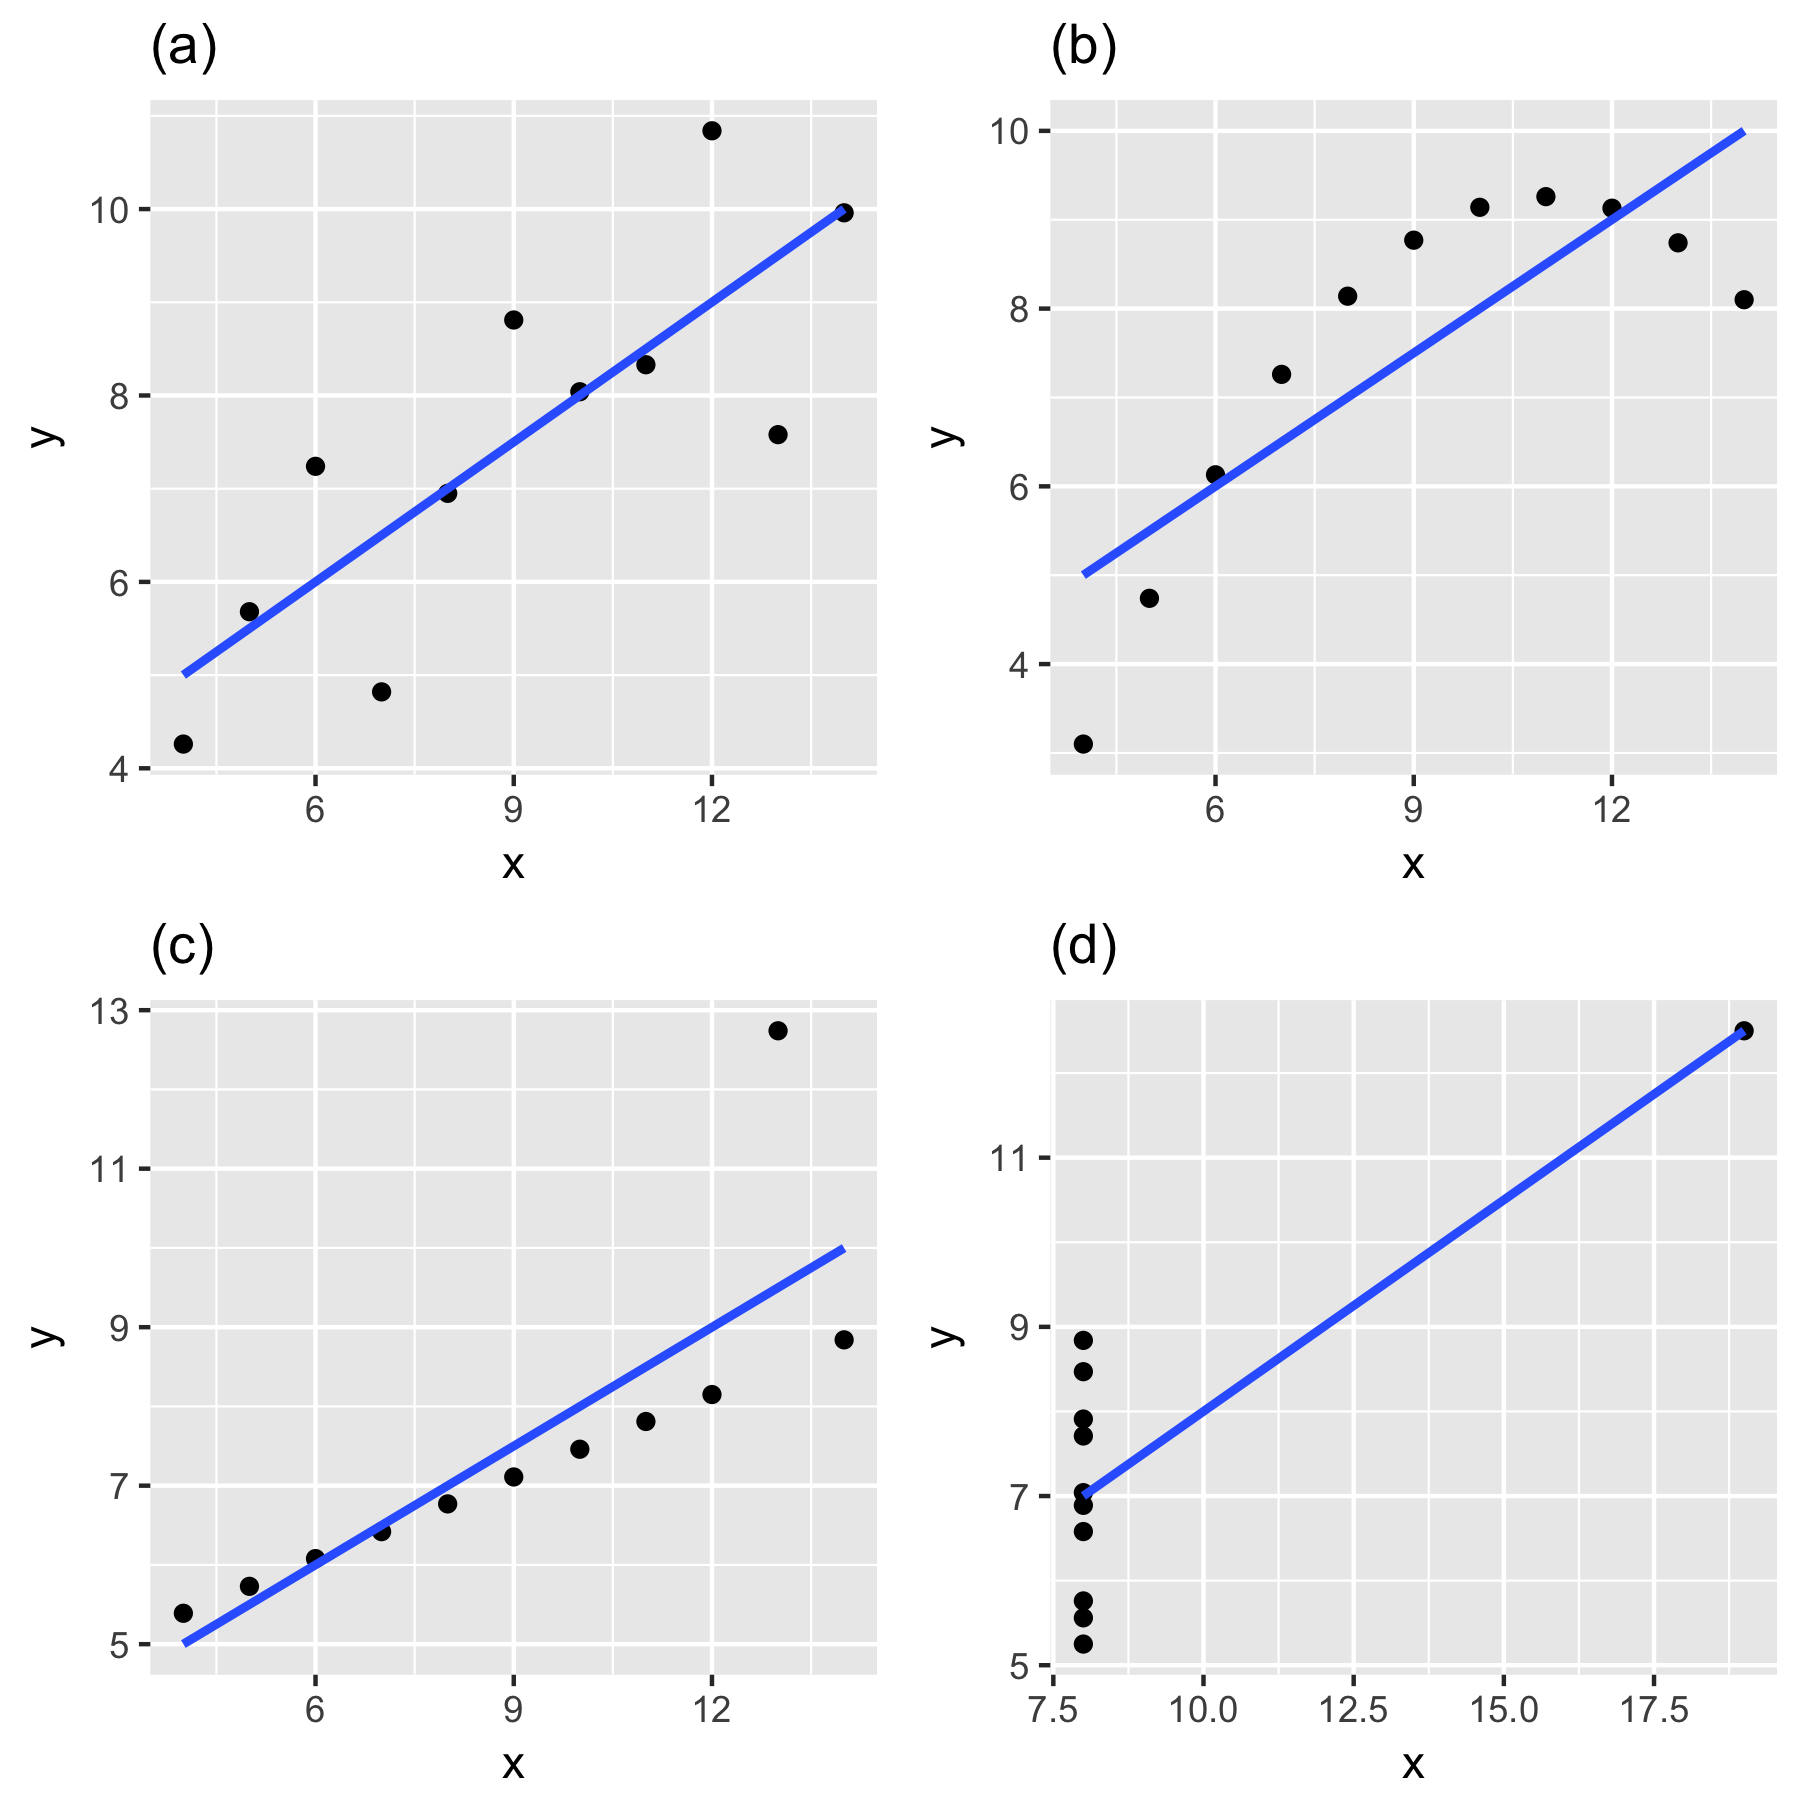
\includegraphics[width=0.7\textwidth]{img/anscombe.png}
\end{center}
We can check these assumptions by examining plots of the residuals vs. fitted values of the model (here the ``fitted value'' of point $i$ means $\hat{y}^{(i)}$). 
\begin{center}
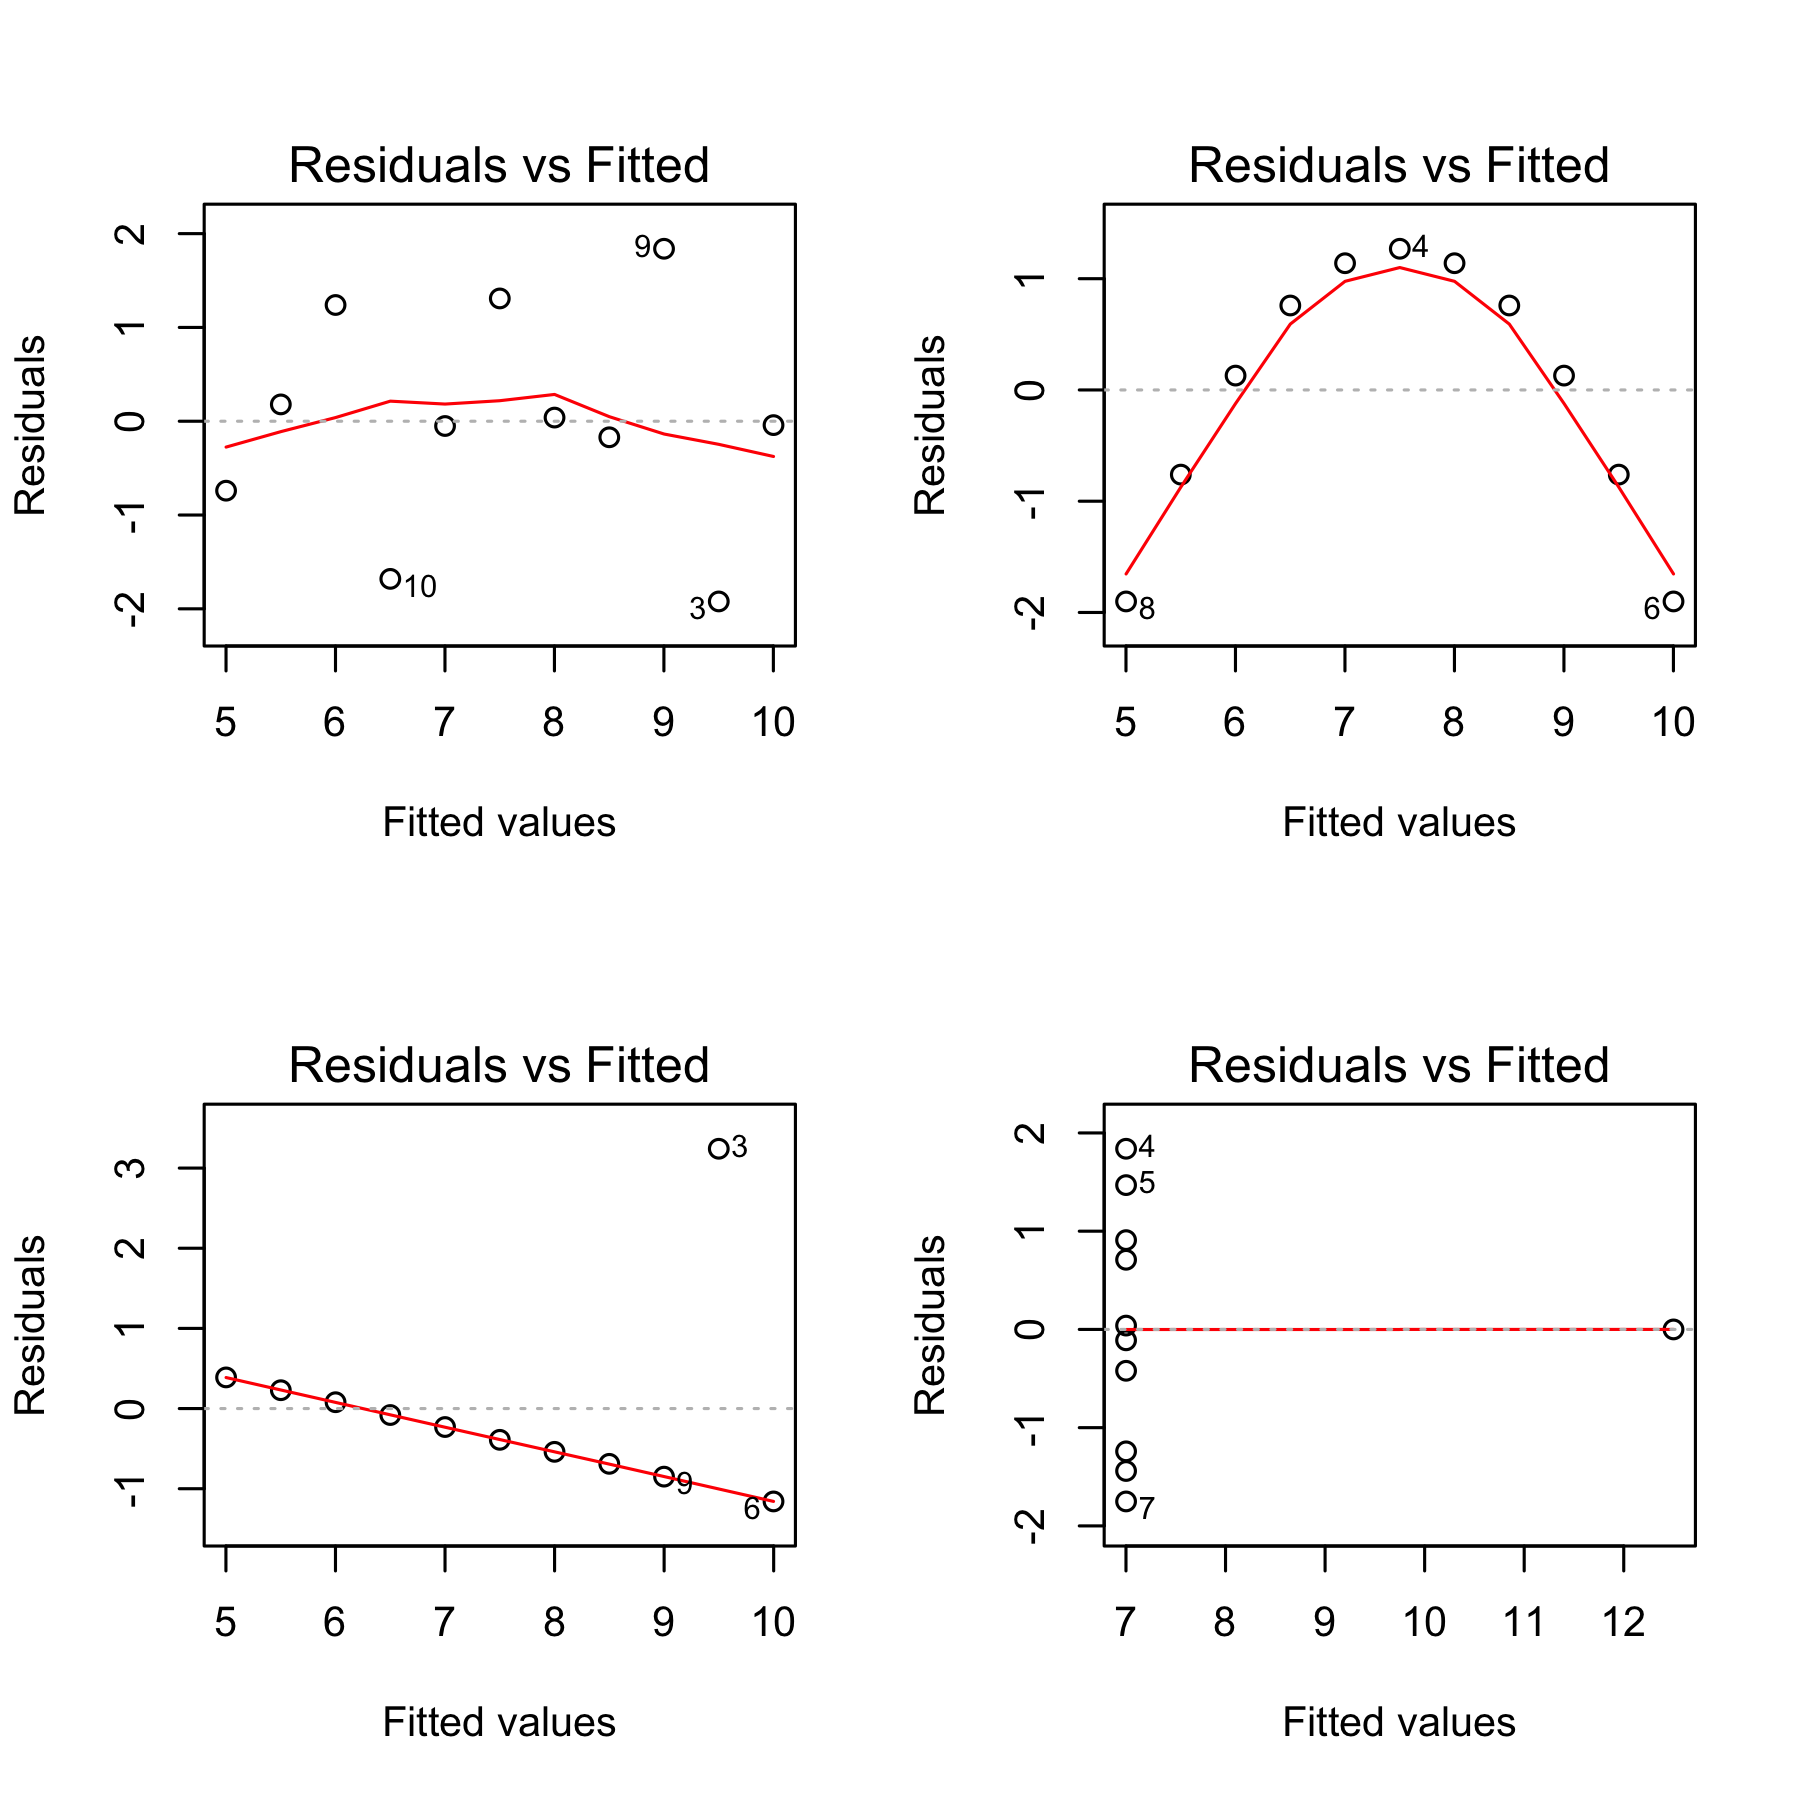
\includegraphics[width=0.7\textwidth]{img/anscombe-diagnostics-1.png}
\end{center}
Which of the four datasets fulfills the assumption of a linear regression model that the error has constant variance? How can you tell?
\end{question}

\subsection{Coefficients and Standard Errors}

Although residuals are important, the parts of the model output that will be scrutinized, reported in papers, etc. are the coefficients, along with their standard errors and hypothesis tests. The coefficients are what create the regression surface, which captures the model's prediction for every point in the feature space (see Section~\ref{ssect:linreg}). 

There are actually a few different ways to derive the coefficients in a linear regression model. The most common way uses \textbf{least squares}, which adjusts the coefficients $\beta_0, \beta_1, \dots, \beta_p$ until the sum of the squared residuals is minimized:
\begin{align*} \text{SSE} &= \sum_{i=1}^n (y^{(i)} - \hat{y}^{(i)})^2 \\
&= \sum_{i=1}^n (y^{(i)} - \beta_0 - \beta_1 x_1^{(i)} - \beta_2 x_2^{(i)} - \dots - \beta_p x_p^{(i)})^2 \end{align*}
It turns out that you can find the optimal values of the $\beta$s analytically by taking derivatives of this thing and setting them equal to zero. Alas, this requires some matrix multiplication and the taking of matrix inverses, so we will save it for a later chapter. Suffice it to say that the $\beta$s are adjusted to minimize the SSE, and the values in the model output are the optimal values.
\vspace{5mm}

\begin{question}{}
Looking at the form of the linear regression model
$$ y = \beta_0 + \beta_1 x_1 + \dots + \beta_p x_p + \varepsilon $$
what does the value of each of the $\beta$s mean? What is $\beta_j$ telling us about how $y$ varies with the predictor $j$, all else being equal?
\end{question}

The model's overall estimate of $\sigma$, the standard deviation of the error term, is obtained very naturally by averaging over the residuals, taking into account the number of predictors, $p$:
$$ \hat{\sigma}^2 = \frac{1}{n-p-1} \sum_{i=1}^n (y^{(i)} - \hat{y}^{(i)})^2.$$

\begin{question}{}
The sum of the squared residuals for our model is $4480.678$. There are $n=200$ datapoints, and the number of predictors, $p$, is 2. Calculate $\hat{\sigma}$ for this model. Do you see this number anywhere in the model output? What is it called?
\end{question}

The standard errors of the model coefficients likewise require matrix multiplication to fully understand, but they are related to three factors: (1) the value of $\hat{\sigma}$, (2) the spread of the values of the corresponding covariate about its mean (more spread will decrease the standard error), and (3) correlations between that covariate and other covariates in the model (tighter correlations will increase the standard error).
\vspace{5mm}

\begin{question}{}
The standard errors attempt to capture how much we expect our estimates of the model coefficients to vary if we were to refit the model using a different dataset, provided that the new dataset is similar to (i.e., sampled from the same population distribution as) the one used to fit the model. On average, approximately how much would we expect $\beta_0$ (the intercept) to deviate from its fitted value of 49.8600? How much would we expect $\beta_1$ and $\beta_2$ to deviate from their fitted values? 
\end{question}

\subsection{Hypothesis Tests of Coefficients}

Armed with our coefficients and standard errors, we can perform a hypothesis test on each regression coefficient. Our null hypothesis in each case will be that the true value of that coefficient is zero: that is, it has no effect on the outcome. Under the null hypothesis that $\beta_j = 0$ and assuming $n$, our number of samples, is large enough, the quantity $\hat{\beta_j}/\text{se}(\hat{\beta}_j)$ will be distributed according to a Student's T distribution (see Chapter~\ref{chapter:probabilitydistributions}, Section~\ref{sect:tdist}) with $n-p-1$ degrees of freedom.
\vspace{5mm}

\begin{question}{}
Sketch the null distributions for the hypothesis tests of our three regression coefficients, $\beta_0$, $\beta_1$, and $\beta_2$. Do you see why the $p$-values for these tests are so low?
\end{question}

\subsection{Other Model Output}

The software also provides some other output. The quantity \textbf{R-squared} is defined as:
\begin{align*} R^2 &= 1 - \frac{\sum_{i=1}^n (y^{(i)} - \hat{y}^{(i)})^2}{\sum_{i=1}^n (y^{(i)} - \overline{y})^2} \\[3mm]
&=  1 - \frac{\sum_{i=1}^n (y^{(i)} - \hat{\beta}^T x^{(i)})^2}{\sum_{i=1}^n (y^{(i)} - \overline{y})^2} \end{align*}
or rather, the proportion of total variance in $y$ explained by the model. The \textbf{adjusted R-squared} is almost exactly the same except it fixes a source of bias in $R^2$, namely that $R^2$ will favor models with more parameters. Adjusted $R^2$ penalizes models with more parameters. It is defined as:
\begin{align*}
 R^2_{\text{adj}} &= 1 - \frac{n-1}{n-p-1} \frac{\sum_{i=1}^n (y^{(i)} - \hat{y}^{(i)})^2}{\sum_{i=1}^n (y^{(i)} - \overline{y})^2} \\[3mm]
 &= 1 - (1 - R^2) \frac{n-1}{n-p-1}
\end{align*}
The \textbf{F-statistic} is the ratio of two variances: the variance in the outcome, $y$, that is explained by the model parameters (``sum of squares of regression'', or SSR) and the residual, or unexplained variance (``sum of squares of error'', or SSE). The corresponding \textbf{F-test} tests the null hypothesis that a model with no independent variables (that is, an intercept-only model with $\beta_1 = 0$ and $\beta_2 = 0$) fits the data as well as our model. The F-statistic follows an $F$ distribution with $p$ and $n-p-1$ degrees of freedom (see Chapter~\ref{chapter:probabilitydistributions}, Section~\ref{sect:fdist}). The $p$-value reported in the model output is the $p$-value for this hypothesis test.  

%%%%%%%%%%%%%%%%%%%%%%%%%%%%%%%%%%%%%%%%%%%%%%%%%%%%%%%%%%%%%%%%%%%%%%%%%%%%%%%%

\section{Example: Small Cities Pollution Dataset}

The following data come from an early study that examined the possible link between air pollution and mortality. The authors examined 60 cities throughout the United States and recorded the following data:
\begin{center}
\texttt{ \small \begin{tabular}{ll}
\toprule
MORT & Total age-adjusted mortality from all causes, \\
& in deaths per 100,000 population \\
PRECIP & Mean annual precipitation (in inches) \\
EDUC & Median number of school years completed \\
& for persons of age 25 years or older \\
NONWHITE & Percentage of the 1960 population that is nonwhite \\
NOX & Relative pollution potential of oxides of nitrogen \\
SO2 & Relative pollution potential of sulfur dioxide \\
\bottomrule
\end{tabular}
}
\end{center}
Note: ``Relative pollution potential'' refers to the product of the tons emitted per day per square kilometer and a factor correcting the SMSA dimensions and exposure.

We want to predict the value of \texttt{MORT} ($y$) using the predictors \texttt{PRECIP, EDUC, NONWHITE, NOX,} and \verb|SO2| ($x_1, x_2, x_3, x_4$ and $x_5$). Here is the output for a fitted linear regression model:
\begin{center}
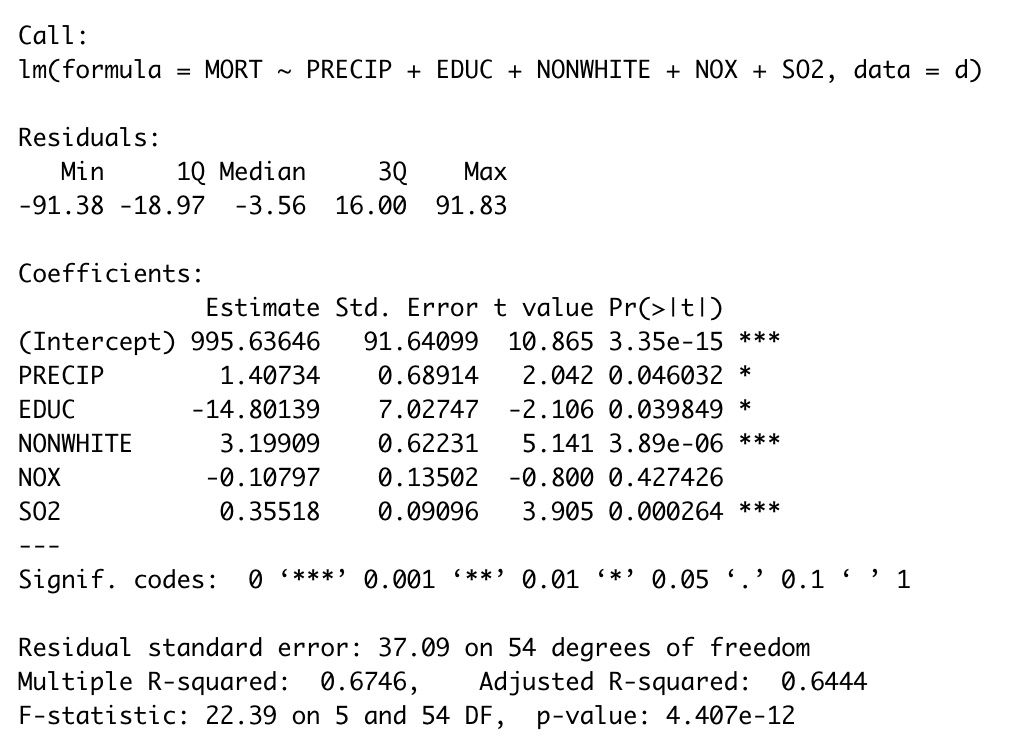
\includegraphics[width=0.8\textwidth]{img/linear-small-cities-model.png}
\end{center}

\begin{question}{}
Interpret the values of each of these coefficients. Based on the coefficient values and their standard errors, which predictor(s) do you think have the greatest impact on mortality? 
\end{question}

\begin{question}{}
In this model, is the effect of one predictor (say, \verb|PRECIP|) impacted by the value(s) of any of the other predictor(s)? How does this differ from the other regression algorithms we've seen (KNN and decision trees)? What are the advantages and disadvantages of this choice? 
\end{question}

\begin{question}{}
Is a normal distribution the right distribution to model an outcome of age-adjusted mortality (MORT)? Why or why not? Look back at our discussion of the normal distribution in Chapter~\ref{chapter:probabilitydistributions} if you need a refresher. 
\end{question}
